\chapter{Fundamentos Geofísicos}

\section{Campo potencial gravitatorio}

Según la Ley de Gravitación Universal de Newton, una masa puntual $m_p$ situada
en la posición $\mathbf{p}$ siente una fuerza gravitatoria $\mathbf{F}$ debido
a la presencia de otra masa $m$ situada en la posición $\mathbf{q}$. Esta
fuerza puede expresarse como:

\begin{equation}
    \mathbf{F} =
        - G \frac{m_p m}{|\mathbf{p} - \mathbf{q}|^3} (\mathbf{p} - \mathbf{q}),
\end{equation}

\noindent donde $G = 6.67430 \times 10^{-11} \text{m}^3 \text{kg}^{-1}
\text{s}^{-2}$ es la constante de gravitación universal
(Fig.~\ref{fig:potencial-gravitatorio}a).
Aplicando la segunda Ley de Newton, se deduce que la masa $m_p$ siente una
aceleración gravitatoria $\mathbf{g}$:

\begin{equation}
    \mathbf{g} =
        - \frac{G m}{|\mathbf{p} - \mathbf{q}|^3} (\mathbf{p} - \mathbf{q}).
    \label{eq:aceleracion-newton}
\end{equation}

Si consideramos que la partícula $m_p$ es una \emph{partícula de prueba},
podemos reescribir la ecuación \ref{eq:aceleracion-newton}, pero ahora
resignificándola como la aceleración gravitatoria que sentiría cualquier
partícula localizada en un punto $\mathbf{p}$ debido a la presencia de la
partícula $m$:

\begin{equation}
    \mathbf{g}(\mathbf{p}) =
        - \frac{G m}{|\mathbf{p} - \mathbf{q}|^3} (\mathbf{p} - \mathbf{q}).
\end{equation}

Se puede demostrar que la atracción gravitatoria $\mathbf{g}$ define un campo
irrotacional, es decir:

\begin{equation}
    \nabla \times \mathbf{g} = 0.
\end{equation}

\noindent Por ende es posible definir un potencial escalar $V$ al que
denominaremos \emph{potencial gravitatorio}:

\begin{equation}
    \mathbf{g}(\mathbf{p}) = + \nabla V(\mathbf{p}),
    \label{eq:potencial-gravitatorio-definicion}
\end{equation}

\noindent donde

\begin{equation}
    V(\mathbf{p}) = G \frac{m}{|\mathbf{p} - \mathbf{q}|}.
    \label{eq:potencial-gravitatorio-particula}
\end{equation}

\noindent Vale la pena notar que en la ecuación
\ref{eq:potencial-gravitatorio-definicion} se ha aplicado la convención de
signo positivo para definir el potencial $V$, mayormente utilizada en la
literatura sobre Geofísica y Geodesia
\citep{heiskanen1967,blakely1995,hinze2009}.

\begin{figure}
    \centering
    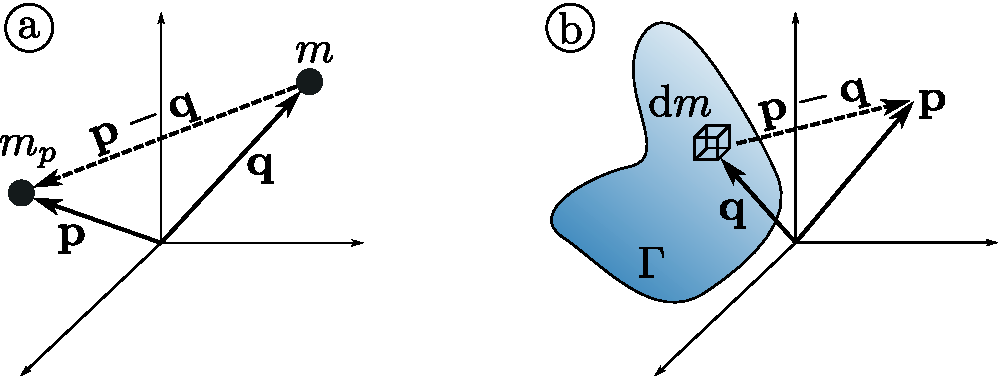
\includegraphics[width=\linewidth]{figs/gravity-potentials.pdf}
    \caption{
        (a)~Masas puntuales $m_p$ y $m$ localizadas en $\mathbf{p}$
        y $\mathbf{q}$, respectivamente.
        (b)~Distribución de masa $\Gamma$, diferencial de masa $\text{d}m$
        ubicado en el punto $\mathbf{q}$.
    }
    \label{fig:potencial-gravitatorio}
\end{figure}


\subsection{Potencial gravitatorio producido por una distribución de masa}

Partiendo de que un diferencial de masa $\text{d}m$ ubicado en $\mathbf{q}$
genera un potencial gravitatorio $\text{d}V$ en cualquier punto $\mathbf{p}$
(Fig.~\ref{fig:potencial-gravitatorio}b):

\begin{equation}
    \text{d}V(\mathbf{p}) = \frac{G}{|\mathbf{p} - \mathbf{q}|} \text{d}m,
\end{equation}

\noindent el potencial gravitatorio generado por una distribución de masa
$\Gamma$ puede calcularse integrando los diferenciales de masa que lo componen:

\begin{equation}
    V(\mathbf{p}) =
        G \int\limits_\Gamma \frac{\text{d}m}{|\mathbf{p} - \mathbf{q}|} .
\end{equation}

Si reescribimos los diferenciales de masa como

\begin{equation}
    \text{d}m = \rho(\mathbf{q}) \text{d}v,
\end{equation}

\noindent donde $\rho(\mathbf{q})$ es la densidad de masa de la distribución
$\Gamma$ en el punto $\mathbf{q}$ y $\text{d}v$ es el diferencial de volumen,
el potencial se puede expresar como:

\begin{equation}
    V(\mathbf{p}) =
        G \int\limits_\Gamma
        \frac{\rho(\mathbf{q})}{|\mathbf{p} - \mathbf{q}|} \text{d}v.
    \label{eq:potencial-gravitatorio-integral}
\end{equation}


\subsection{Gradiente del potencial gravitatorio}

Según la definición del potencial gravitatorio expuesta en la
ecuación~\ref{eq:potencial-gravitatorio-definicion}, es posible calcular la
aceleración de la gravedad producida por una distribución de masa arbitraria
en cualquier punto $\mathbf{p}$ como el gradiente del potencial
$V(\mathbf{p})$.
Si definimos un sistema de ejes Cartesianos en el cual el punto $\mathbf{p}
= (x, y, z)$, las componentes de la aceleración en cada una de las direcciones
del sistema quedan expresadas
como:

\begin{equation}
    g_i(\mathbf{p}) = \frac{\partial V(\mathbf{p})}{\partial i}, \,\,
        \forall i \in \{x, y, z\}.
    \label{eq:componentes-aceleracion-gravitatoria}
\end{equation}

El vector
$\mathbf{g}(\mathbf{p}) = (g_x(\mathbf{p}), g_y(\mathbf{p}), g_z(\mathbf{p}))$
representa la aceleración gravitatoria en el punto
$\mathbf{p}$ generada por la distribución de masa $\Gamma$, aunque es común
referirse al mismo como el \emph{gradiente gravitatorio}.
Reemplazando la ecuación~\ref{eq:potencial-gravitatorio-integral}
en~\ref{eq:componentes-aceleracion-gravitatoria}, las componentes del gradiente
gravitatorio pueden expresarse como:

\begin{align}
    g_x(\mathbf{p}) =&
        - G \int\limits_\Gamma \rho(\mathbf{q})
        \frac{(x - x')}{|\mathbf{p} - \mathbf{q}|^3} \text{d}v,
    \label{eq:gx-integral}
    \\
    g_y(\mathbf{p}) =&
        - G \int\limits_\Gamma \rho(\mathbf{q})
        \frac{(y - y')}{|\mathbf{p} - \mathbf{q}|^3} \text{d}v,
    \label{eq:gy-integral}
    \\
    g_z(\mathbf{p}) =&
        - G \int\limits_\Gamma \rho(\mathbf{q})
        \frac{(z - z')}{|\mathbf{p} - \mathbf{q}|^3} \text{d}v,
    \label{eq:gz-integral}
\end{align}

\noindent donde $\mathbf{q} = (x', y', z')$.

Las segundas derivadas del potencial gravitatorio definen el \emph{tensor del
gradiente gravitatorio}, y sus componentes pueden expresarse como:

\begin{equation}
    g_{ij}(\mathbf{p}) =
        \frac{\partial^2 V(\mathbf{p})}{\partial i \partial j}, \,\,
        \forall i \in \{x, y, z\}, \,\,
        \forall j \in \{x, y, z\}.
\end{equation}

Reemplazando la ecuación \ref{eq:potencial-gravitatorio-integral}, podemos
expresar las componentes diagonales del tensor de la siguiente manera
\citep{grombein2013}:

\begin{align}
    g_{xx}(\mathbf{p}) =&
        G \int\limits_\Gamma \rho(\mathbf{q})
        \left[
        \frac{3(x - x')^2}{|\mathbf{p} - \mathbf{q}|^5}
        - \frac{1}{|\mathbf{p} - \mathbf{q}|^3}
        \right]
        \text{d}v,
    \label{eq:gxx-integral}
    \\
    g_{yy}(\mathbf{p}) =&
        G \int\limits_\Gamma \rho(\mathbf{q})
        \left[
        \frac{3(y - y')^2}{|\mathbf{p} - \mathbf{q}|^5}
        - \frac{1}{|\mathbf{p} - \mathbf{q}|^3}
        \right]
        \text{d}v,
    \label{eq:gyy-integral}
    \\
    g_{zz}(\mathbf{p}) =&
        G \int\limits_\Gamma \rho(\mathbf{q})
        \left[
        \frac{3(z - z')^2}{|\mathbf{p} - \mathbf{q}|^5}
        - \frac{1}{|\mathbf{p} - \mathbf{q}|^3}
        \right]
        \text{d}v,
    \label{eq:gzz-integral}
\end{align}

\noindent mientras que las componentes no diagonales pueden expresarse como:

\begin{align}
    g_{xy}(\mathbf{p}) =
    g_{yx}(\mathbf{p}) =&
        G \int\limits_\Gamma \rho(\mathbf{q})
        \frac{3(x - x')(y - y')}{|\mathbf{p} - \mathbf{q}|^5}
        \text{d}v,
    \label{eq:gxy-integral}
    \\
    g_{xz}(\mathbf{p}) =
    g_{zx}(\mathbf{p}) =&
        G \int\limits_\Gamma \rho(\mathbf{q})
        \frac{3(x - x')(z - z')}{|\mathbf{p} - \mathbf{q}|^5}
        \text{d}v,
    \label{eq:gxz-integral}
    \\
    g_{yz}(\mathbf{p}) =
    g_{zy}(\mathbf{p}) =&
        G \int\limits_\Gamma \rho(\mathbf{q})
        \frac{3(y - y')(z - z')}{|\mathbf{p} - \mathbf{q}|^5}
        \text{d}v.
    \label{eq:gyz-integral}
\end{align}

A partir de las ecuaciones~\ref{eq:gxx-integral}--\ref{eq:gzz-integral} podemos
calcular el Laplaciano del potencial gravitatorio:

\begin{equation}
    \Delta V(\mathbf{p}) = \nabla^2 V(\mathbf{p}) =
        \frac{\partial^2 V}{\partial x^2}
        + \frac{\partial^2 V}{\partial y^2}
        + \frac{\partial^2 V}{\partial z^2},
\end{equation}

\noindent Dado que las tres expresiones se cancelan mutuamente
\citep{blakely1995}, podemos concluir que cualquier potencial gravitatorio es
un \emph{campo harmónico}

\begin{equation}
    \Delta V(\mathbf{p}) = 0
\end{equation}

\noindent para cualquier punto de observación $\mathbf{p}$.

% =============================================================================

\section{Modelado directo}

El cálculo de los efectos gravitatorios de un determinado cuerpo sobre uno
o más puntos de observación se suele denominar modelado directo (\emph{forward
modelling} en inglés).
Aunque las expresiones del potencial gravitatorio
(ec.~\ref{eq:potencial-gravitatorio-integral}),
las componentes de su gradiente
(ecs.~\ref{eq:gx-integral}--\ref{eq:gz-integral})
y de su tensor (ecs.~\ref{eq:gxx-integral}--\ref{eq:gzz-integral}
aparentan ser sencillas, el cómputo de estas magnitudes para una geometría dada
no resulta un problema trivial.
Solo existen soluciones analíticas a dichas expresiones para determinadas
geometrías sencillas o que guardan algún tipo de simetría.

En el desarrollo de esta Tesis nos resultan de principal interés trabajar con
tres tipos de geometrías: masas puntuales, prismas rectangulares y prismas
esféricos o \emph{tesseroides}.

\subsection{Masas puntuales}

La distribución de densidades de una masa puntual puede expresarse
sencillamente mediante una Delta de Dirac \citep{vladimirov1979}:

\begin{equation}
    \rho(\mathbf{q}) = m \, \delta(\mathbf{q} - \mathbf{q'}),
\end{equation}

\noindent donde $\mathbf{q}$ y $m$ son la posición y la masa de la partícula,
respectivamente.
Reemplazando esta expresión en la
ecuación~\ref{eq:potencial-gravitatorio-integral}, obtenemos el potencial
gravitatorio generado por una partícula:

\begin{equation}
    V(\mathbf{p}) =
        G \int\limits_\Gamma
        m \frac{\delta(\mathbf{q} - \mathbf{q'})}{|\mathbf{p} - \mathbf{q'}|}
        \text{d}v =
        \frac{G m}{|\mathbf{p} - \mathbf{q}|},
    \label{eq:potencial-masa-puntual}
\end{equation}

\noindent de acuerdo con la expresión del potencial de la
ecuación~\ref{eq:potencial-gravitatorio-particula}.

Realizando el mismo reemplazos en las ecuaciones correspondientes a las
componentes del gradiente (ecs.~\ref{eq:gx-integral}--\ref{eq:gz-integral})
arribamos a las siguientes expresiones:

\begin{align}
    g_x(\mathbf{p}) =&
        - G m
        \frac{x - x'}{|\mathbf{p} - \mathbf{q}|^3},
    \label{eq:gx-particula}
    \\
    g_y(\mathbf{p}) =&
        - G m
        \frac{y - y'}{|\mathbf{p} - \mathbf{q}|^3},
    \label{eq:gy-particula}
    \\
    g_z(\mathbf{p}) =&
        - G m
        \frac{z - z'}{|\mathbf{p} - \mathbf{q}|^3}.
    \label{eq:gz-particula}
\end{align}

A la hora de realizar el cómputo de los campos gravitatorios de masas
puntuales, las posiciones de las partículas como de los puntos de observación
pueden venir dados en diferentes sistemas de coordenadas.
En el caso de necesitar modelar cualquier conjunto de masas situadas bajo la
superficie terrestre, resulta natural utilizar coordenadas esféricas tanto para
las posiciones de las partículas como para los puntos de observación.
Sin embargo, es muy común trabajar sobre zonas de estudio con dimensiones
acotadas, bajo las cuales la aproximación de tierra plana es suficiente. En
estos casos es posible trabajar en coordenadas Cartesianas.

\subsubsection{Coordenadas Cartesianas}

En el caso de que la posición de la partícula venga dada por el vector
$\mathbf{q} = (x', y', z')$ y el punto de observación por el vector
$\mathbf{p} = (x, y, z)$ definidos en el mismo sistema de ejes Cartesianos, el
módulo de
$\mathbf{p} - \mathbf{q}$ se calcula sencillamente bajo la norma L$_2$:

\begin{equation}
    | \mathbf{p} - \mathbf{q} | = \sqrt{
        (x - x')^2 + (y - y')^2 + (z - z')^2
    }.
\end{equation}

Dado que los numeradores en las
ecuaciones~\ref{eq:gx-particula}--\ref{eq:gz-particula} resultan triviales en
coordenadas Cartesianas, el cómputo del potencial y las componentes de su
gradiente se puede realizar de manera sencilla.

\subsubsection{Coordenadas esféricas}

Consideremos que las posiciones del punto de observación y de la partícula
vienen dados en un sistema de coordenadas esféricas. Para ello vamos a definir
un sistema de referencia \emph{geocéntrico} $\{X, Y, Z\}$ y a partir del mismo
un sistema de coordenadas esféricas $\{r, \lambda, \phi\}$, donde $r$ es la
posición \emph{radial}, $\lambda$ la posición \emph{longitudinal} y $\phi$ la
posición \emph{latitudinal} (Fig.~\ref{fig:spherical-coordinates}).
Cualquier punto dado por las coordenadas esféricas $(r, \lambda, \phi)$ se
puede expresar en coordenadas Cartesianas geocéntricas bajo las siguientes
relaciones:

\begin{equation}
    \begin{cases}
        X = r \cos\lambda \cos{\phi} \\
        Y = r \sin\lambda \cos{\phi} \\
        Z = r \sin{\phi},
    \end{cases}
\end{equation}

\noindent donde $r \in [0, \infty)$, $\lambda \in (-\pi, \pi]$ y
$\phi \in [-\pi/2, \pi/2]$.

\begin{figure}
    \centering
    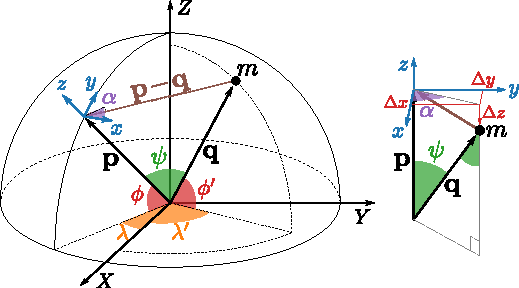
\includegraphics[width=\linewidth]{figs/spherical-coordinates.pdf}
    \caption{
        Masa puntual $m$ ubicada en la posición $\mathbf{q}$ y punto de
        observación situado en $\mathbf{p}$.
        Se define un sistema de referencia Cartesiano \emph{geocéntrico} $X, Y,
        Z$ bajo el cual se considera un sistema de coordenadas esféricas dadas
        por la distancia radial ($r$), ángulo longitudinal ($\lambda$) y ángulo
        latitudinal ($\phi$).
        En el punto $\mathbf{p}$ se define un sistema \emph{local} de
        coordenadas Cartesiano: el eje $x$ apunta hacia el Este,
        el eje $y$ hacia el Norte geométrico y el eje $z$ en la dirección
        radial.
        Se define a $\psi$ como el ángulo descripto por los vectores
        $\mathbf{p}$ y $\mathbf{q}$, y $\alpha$ al ángulo azimutal de
        $-(\mathbf{p} - \mathbf{q})$ sobre el sistema \emph{local}.
    }
    \label{fig:spherical-coordinates}
\end{figure}

El potencial gravitatorio que genera la partícula $m$ sobre el punto de
observación $\mathbf{p}$ puede calcularse mediante la
ecuación~\ref{eq:potencial-gravitatorio-particula}.
Considerando que los vectores $\mathbf{p}$ y $\mathbf{q}$ vienen definidos por
las coordenadas esféricas $(r, \lambda, \phi)$ y $(r', \lambda', \phi')$,
respectivamente, la distancia Euclidiana entre ellos puede expresarse como
\citep{grombein2013}:

\begin{equation}
    |\mathbf{p} - \mathbf{q}| = \sqrt{
        r^2 + r'^2 - 2rr'\cos\psi
    },
    \label{eq:distance-spherical}
\end{equation}

\noindent donde $\psi$ es el ángulo que describen los vectores $\mathbf{p}$
y $\mathbf{q}$:

\begin{equation}
    \cos \psi =
        \sin \phi \sin \phi' + \cos \phi \cos \phi' \cos(\lambda - \lambda').
    \label{eq:cosphi}
\end{equation}

La determinación de las componentes del gradiente del potencial gravitatorio
hace necesario que definamos las direcciones ortogonales $x$, $y$ y $z$ a lo
largo de las cuales se calculan las derivadas parciales de $V(\mathbf{p})$.
La elección más natural es obtener el gradiente con respecto a un sistema de
coordenadas \emph{local} $\{x, y, z\}$ \citep{grombein2013,uieda2016} donde $x$
se orienta en la dirección longitudinal (Este), $y$ en la dirección latitudinal
(Norte) y $z$ en la dirección radial.

Los numeradores de las ecuaciones~\ref{eq:gx-particula}--\ref{eq:gz-particula}
pueden expresarse en términos de las coordenadas esféricas como:

\begin{align}
    \Delta x =& - (x - x') = r' \sin\psi \cos\alpha
    \label{eq:delta-x-raw}
    \\
    \Delta y =& - (y - y') = r' \sin\psi \sin\alpha
    \label{eq:delta-y-raw}
    \\
    \Delta z =& - (z - z') = r'\cos\psi - r,
    \label{eq:delta-z-raw}
\end{align}

\noindent donde $\alpha$ es el ángulo azimutal del vector
$-(\mathbf{p} - \mathbf{q})$ sobre el sistema de coordenadas \emph{locales}.
Haciendo uso de las siguientes relaciones de trigonometría esférica
\citep[][p.~113]{heiskanen1967}:

\begin{align}
    \sin\psi \cos\alpha =&
        \cos\phi \sin\phi' - \sin\phi \cos\phi' \cos(\lambda - \lambda') \\
    \sin\psi \sin\alpha =&
        \cos\phi' \sin(\lambda - \lambda'),
\end{align}

\noindent podemos expresar las ecuaciones~\ref{eq:delta-x-raw},
\ref{eq:delta-y-raw} y \ref{eq:delta-z-raw} como \citep{grombein2013}:

\begin{align}
    \Delta x =& r' \sin\psi \left[
        \cos\phi \sin\phi' - \sin\phi \cos\phi' \cos(\lambda - \lambda')
        \right]
    \label{eq:delta-x}
    \\
    \Delta y =& r' \cos\phi' \sin(\lambda - \lambda')
    \label{eq:delta-y}
    \\
    \Delta z =& r'\cos\psi - r.
    \label{eq:delta-z}
\end{align}

De esta forma podemos expresar las componentes del gradiente del potencial
gravitatorio generado por una masa puntual en coordenadas esféricas como:

\begin{align}
    g_x(\mathbf{p}) =&
        G m
        \frac{\Delta x}{|\mathbf{p} - \mathbf{q}|^3},
    \label{eq:gx-particula-spherical}
    \\
    g_y(\mathbf{p}) =&
        G m
        \frac{\Delta y}{|\mathbf{p} - \mathbf{q}|^3},
    \label{eq:gy-particula-spherical}
    \\
    g_z(\mathbf{p}) =&
        G m
        \frac{\Delta z}{|\mathbf{p} - \mathbf{q}|^3},
    \label{eq:gz-particula-spherical}
\end{align}

\noindent haciendo uso de las ecuaciones~\ref{eq:distance-spherical},
\ref{eq:cosphi}, \ref{eq:delta-x}, \ref{eq:delta-y} y \ref{eq:delta-z}.


\subsection{Prismas rectangulares}

\subsection{Tesseroides}

% =============================================================================

\section{Disturbio de gravedad}

\subsection{Elipsoide de referencia}

\section{Fuentes equivalentes}
